\section{Graphical Interfaces}

\lstdefinestyle{DOS}
{
	backgroundcolor=\color{black},
	basicstyle=\footnotesize\color{white}\ttfamily
	identifierstyle=\color{white}
	commentstyle=\color{white},
	keywordstyle=\color{white},
	stringstyle=\color{white},
	frame=lines,
	keepspaces=true,
	numbers=none,
	aboveskip=0\baselineskip
}

Scientific programming is often focused on creating a model, a simulation or a digital twin of a chemical or physical process, or on control of an otherwise unstable system. For many cases, the program can operate in the background or read input and yield output via a file, a console or low-level communication protocols. However, a scientific program may be more convincing when input and output is visible in a \emph{graphical interface}, together with a graphical representation of the progress of the calculations. The construction of such interfaces is the topic of this Chapter. 

\subsection{Sequential vs. event-driven programs}

The earliest computer programs all show a \emph{sequential} structure. Input is read from the first few program lines or from a file on disk. Calculations are performed and finally the results are printed to paper, a console or an output file on disk. This type of program is easily understood when coded line-by line on \href{https://en.wikipedia.org/wiki/Punched_card}{\emph{punched cards}}. The basic idea is found in the \href{https://en.wikipedia.org/wiki/Turing_machine}{Turing machine}, invented in 1936 by \href{https://en.wikipedia.org/wiki/Alan_Turing}{Alan Turing}.
For \href{https://en.wikipedia.org/wiki/Fortran}{FORTRAN} programs, this programming style is still in use. This is due to the availability of very reliable code and compilers in this language, together with high-speed execution of the compiled code.
An answer to the question  \href{https://www.researchgate.net/post/How_can_I_create_a_Graphical_User_Interface_for_FORTRAN_code}{How can I create a Graphical User Interface for FORTRAN code?} will inevitably lead to other computer languages like C++ and Python. For these languages, graphical frameworks have been made, that take advantage of the Graphical User Interface (GUI) of the operating system of the computer. Program control is done via pushbuttons, check boxes, operated by mouse clicks or gestures. Each key press action or operation of the mouse is called an \emph{event}. Upon each event, a calculation or any other pre-defined part of the program code is executed. In between, the program idles in an \emph{event loop}. This summarizes the \emph{event-driven} programming style.  

Further information can be found in \href{https://en.wikipedia.org/wiki/Comparison_of_programming_paradigms}{programming paradigms}.

\subsection{Graphical frameworks}

Graphical frameworks or \href{https://en.wikipedia.org/wiki/List_of_platform-independent_GUI_libraries}{GUI libraries} exist for all operating systems (OSes). In this manual, we will use the \href{https://en.wikipedia.org/wiki/Qt_(software)}{Qt} framework, originally developed by Nokia, currently owned by Microsoft. This framework exists for Windows, Linux, MacOS and also for Android and iOS. Smartphones do not operate without a GUI, whereas other computers have the option of a \emph{console, shell} or \emph{command prompt, PowerShell} for keyboard-only interaction.
The common elements of graphical frameworks are derived from a common denominator of most OSes. The basic element is a \emph{widget}, a screen element that enables mouse interaction.
A \emph{window} is a widget, however it usually encapsulates a group of control widgets. Many programs nowadays show a single-window with multiple control widgets. Some widgets only provide a \emph{display} function for an image, a graph or a movie. The distinction between display and control widgets is very sharp in \emph{e.g.} NI-LabView, but less clear in other frameworks. Widget names for basic elements like pushbuttons differ somewhat between frameworks, but this does not often lead to confusion.

\subsection{Python GUIs}

In Python, the advantage is that the programming language itself is OS-independent. Therefore, graphical frameworks for Python are also universal. The oldest framework for Python is \textsf{\href{https://docs.python.org/3/library/tkinter.html}{tkinter}}, a Python interface to \textsf{Tcl/\href{https://en.wikipedia.org/wiki/Tk_(software)}{Tk}}. A newer option is the Qt framework. A comparison is given in  \href{https://www.pythonguis.com/faq/pyqt-vs-tkinter/}{Qt \emph{vs.} tkinter} Considerations for \href{https://www.pythonguis.com/faq/which-python-gui-library/}{choosing} are discussed on the site \href{https://www.pythonguis.com/}{PythonGUIs} as well.

\subsection{Flavours of Qt in Python}

Navigating the site \href{https://www.pythonguis.com/}{PythonGUIs} may seem a bit cumbersome at first. Several pages are devoted to the differences between \href{https://en.wikipedia.org/wiki/PyQt}{PyQt} and \href{https://en.wikipedia.org/wiki/PySide}{PySide}. Moreover, there have been three releases so far: PyQt4/PySide, PyQt5/PySide2 and PyQt6/PySide6. They implement the main releases of Qt4, Qt5 and Qt6. The syntax differences between PyQt and PySide are reflected in multiple pages covering the different flavours and versions. A basic discussion is given in \href{https://www.pythonguis.com/faq/pyqt5-vs-pyqt6/}{PyQt5 vs. PyQt6} and \href{https://www.pythonguis.com/faq/pyside2-vs-pyside6/}{PySide2 vs. PySide6} and \href{https://www.pythonguis.com/faq/which-python-gui-library/}{choosing}.

it is worth noting that PyQt6 and PySide6 are \emph{Python  bindings} of exactly the same Qt code in C++. The differences originate from the Python implementation only.
In the following sections we will use the Qt6 framework, with PySide6 bindings.

\subsection{Qt installation}

The Qt framework is installed as a Python package. The latest versions are installed in your conda environment with \textsf{pip}:

\begin{lstlisting}[style=DOS]
	pip install pyside6
\end{lstlisting}
or 
\begin{lstlisting}[style=DOS]
	pip install pyqt6
	pip install pyqt6-tools
\end{lstlisting}

Note that \textsf{conda install} is not used here. The \textsf{conda} packages for Qt6 are currently incomplete or absent.

\subsection{A basic Qt program}

In its simplest form, a Python script with GUI looks as follows:
\begin{lstlisting}[language=Python, numbers=none, aboveskip=\smallskipamount]
	import sys
	from PySide6.QtWidgets import QApplication, QMainWindow
	
	app = QApplication()
	window = QMainWindow()
	window.show()
	sys.exit(app.exec())
\end{lstlisting}
After creation of a QApplication and a QMainWindow \emph{widget}, this script shows an empty window, according to the default settings of the OS. The window handles are functional, but other functions have yet to be implemented. The program enters the \emph{event loop} with \textsf{app.exec()}, waiting for mouse or keyboard interaction. Upon closing the window, the event loop is terminated, with exit code \textsf{0}. The 
\href{https://superfastpython.com/exit-process/#What_is_sysexit}{\textsf{sys.exit()}} command displays this exit code.

\subsection{A minimal Qt program with a useful QMainWindow widget}

In practice, the programmer wants to design his or her own GUI. This can be achieved by \emph{subclassing} the QMainWindow class, adding a title, resizing and adding \emph{widgets}. The example below adds a QPushButton widget which occupies the entire window.

The basic code from the previous example is executed in a \textsf{if \_\_name\_\_ == "\_\_main\_\_":} clause. The window is now an instance of the subclass \textsf{MyMainWindow}:

\begin{lstlisting}[language=Python, numbers=none, aboveskip=\smallskipamount]
    import sys
    from PySide6.QtWidgets import QApplication, QMainWindow, QPushButton

    class MyMainWindow(QMainWindow):
        def __init__(self):
        super().__init__()
        self.setWindowTitle("My Program")
        self.setGeometry(300, 300, 300, 200)
        self.button = QPushButton("Click Me!", self)
        self.setCentralWidget(self.button)

    if __name__ == "__main__":
        app = QApplication()
        window = MyMainWindow()
        window.show()
        sys.exit(app.exec())
\end{lstlisting}

Please note, that meaningful GUI programming in Python requires adaptation to the \emph{object-oriented} programming style. Consult \href{https://www.pythonguis.com/tutorials/pyside6-creating-your-first-window/}{First window} for a very similar example.

\subsection{Layout of a GUI in Qt}

In principle, it is possible to build a complete Python GUI by subclassing QMainWindow and add all necessary widgets manually. However, it is easier to use the 
\href{https://www.pythonguis.com/installation/install-qt-designer-standalone/}{QtDesigner} program, which is included in the \textsf{PySide6} package. the program is invoked via the command line interface (CLI) \emph{i.e.} Anaconda Command Prompt or Linux bash shell:

\begin{lstlisting}[style=DOS]
	pyside6-designer
\end{lstlisting}
or
\begin{lstlisting}[style=DOS]
	pyqt6-tools designer
\end{lstlisting}

The default opening screen of QtDesigner is shown in Figure~\ref{fig:qtdesigner}. It offers a choice for constructing a MainWindow, Dialogs with different standard button configurations, or a plain empty widget. Under "Widgets" some further choices for standard widgets are listed, of which the Frame widget is the most relevant option.

\begin{figure}[ht]
	\centering
	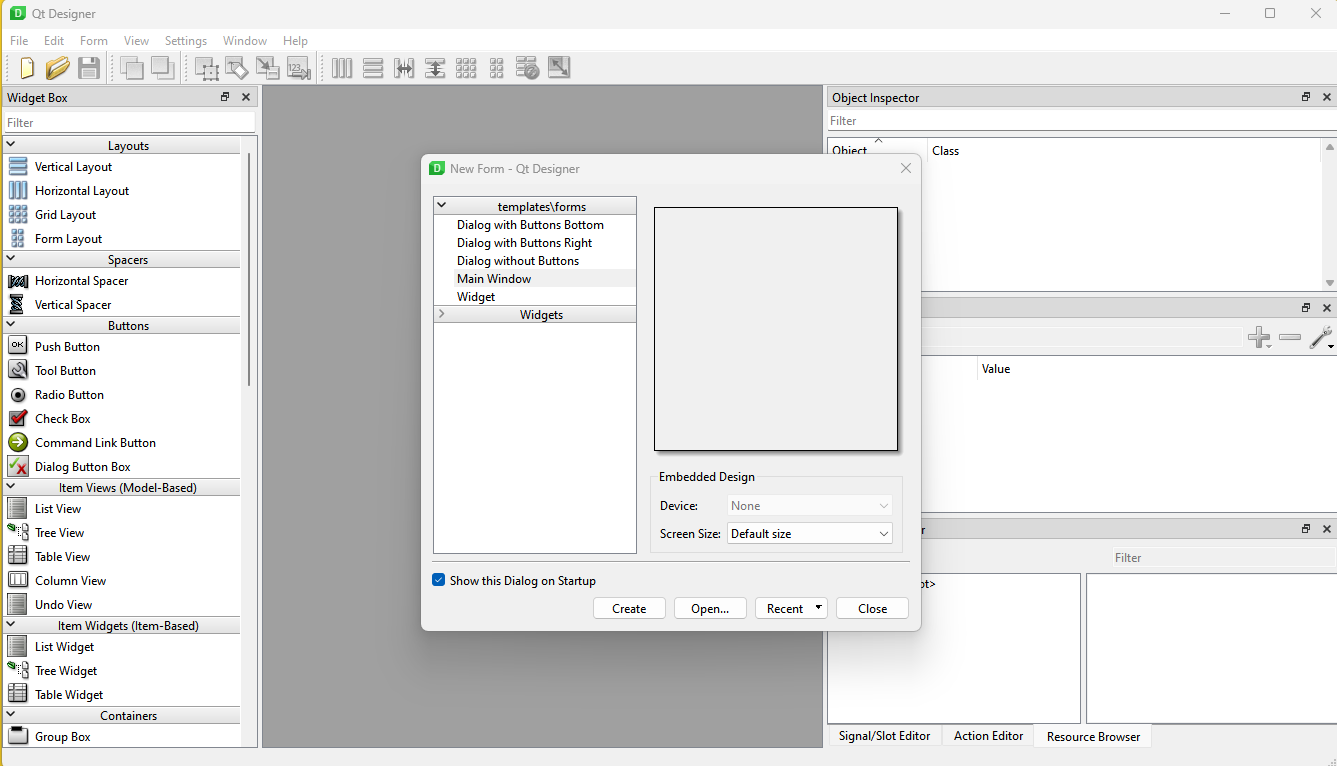
\includegraphics[width=0.7\textwidth]{Figures/QtDesigner.png}
	\caption{QtDesigner program for GUI development}
	\label{fig:qtdesigner}
\end{figure}
Unfortunately, a detailed explanation of the use of QtDesigner in PySide6 is missing on \href{https://www.pythonguis.com/}{PythonGUIs}.  In the \href{https://www.pythonguis.com/tutorials/pyside6-first-steps-qt-designer/}{QtDesigner tutorial}, the program QtCreator is used. See if you can apply the tips for QtCreator in Qtdesigner. Instead, the "official" PySide6 documentation can also be used. See:
\href{https://doc.qt.io/qtforpython-6/tutorials/basictutorial/uifiles.html}{Basic Tutorial}.

\begin{itemize}
	\item create a MainWindow in QtDesigner with a QPusButton, a QCheckbox and a QPlainTextEdit widget.
	\item save the design under the name mymainwindow.ui. 
\end{itemize}
The extension of a file generated by QtDesigner is \textsf{*.ui}. It is written in XML format. You can open it with a text editor and if you are proficient in XML, it will make sense. Otherwise, have faith.

For using the *.ui file in Python, it has to be converted to a *.py file. We follow Option A in the official tutorial.

\begin{lstlisting}[style=DOS]
	pyside6-uic mainwindow.ui -o ui_mainwindow.py
\end{lstlisting}

The generated *.py file contains all the typework you have had to do yourself manually, in Python.

Now the program becomes:
\begin{lstlisting}[language=Python, numbers=none, aboveskip=\smallskipamount]
    import sys
    from PySide6.QtWidgets import QApplication, QMainWindow
    from ui_mainwindow import Ui_MainWindow

    class MyMainWindow(QMainWindow):
    def __init__(self):
        super().__init__()
        self.ui = Ui_MainWindow()
        self.ui.setupUi(self)
        self.setWindowTitle("My Program")

if __name__ == "__main__":
    app = QApplication(sys.argv)
    window = MyMainWindow()
    window.show()
    sys.exit(app.exec())
\end{lstlisting}

In the \textsf{import} section, there is an extra line for import of the graphical class \textsf{Ui\_MainWindow} from the *.py file generated by the program \textsf{pyside6-uic}.

This \textsf{Ui\_MainWindow} class is instantiated into an \emph{attribute} of \textsf{MyMainWindow}

The graphical interface is set up with a call to the \textsf{setupUI} method, which you will find in \textsf{ui\_mainwindow.py}. The argument "self" refers to your MyMainWindow class, which becomes the \emph{parent} class of the \textsf{Ui\_MainWindow} object.

\newpage
